%!TEX program = xelatex
% Note: this template must be compiled with XeLaTeX rather than PDFLaTeX
% due to the custom fonts used. The line above should ensure this happens
% automatically, but if it doesn't, your LaTeX editor should have a simple toggle
% to switch to using XeLaTeX.

\documentclass[
  aspectratio=169, % Uncomment to use an aspect ratio of 16:9 (160 mm by 90 mm)
  %aspectratio=43, % Uncomment to use an aspect ratio of 4:3 (128mm by 96mm)
  t, % Top align all slide content by default
  onlytextwidth, % Typeset content in columns at text width
  10pt, % Default font size, use 10pt for the 16:9 aspect ratio and 8pt for the 4:3 aspect ratio
]{beamer}

\usepackage{../../ImperialTheme/beamer/beamerthemeImperial} % Use the Imperial theme
\usepackage{tikz}
\usetikzlibrary{calc}

\def\imagefolder{../../ImperialTheme/beamer/Images}
\def\Rey{\text{Re}}
\title{Sharpen stability curve} % Presentation title to appear on the title slide and left footers

\subtitle{} % Presentation subtitle to appear on the title slide

\author{Víctor Ballester} % Author name(s) to appear on the title slide

\date{\today} % Presentation date to appear on the title slide and right footers

\begin{document}

\begingroup
\setbeamercolor{background canvas}{bg=ICLLightGrey} % Slide background color
\setbeamercolor{title page title}{fg=ICLBlue} % Title text color
\setbeamercolor{title page subtitle}{fg=ICLBlue} % Subtitle text color
\setbeamercolor{author}{fg=ICLBlue} % Author(s) text color
\setbeamercolor{date}{fg=ICLBlue} % Date text color
\setbeamertemplate{title page}[logo]{\imagefolder/ICL_Logo_Blue.pdf} % Imperial logo color, use 'ICL_Logo_White.pdf' for white and 'ICL_Logo_Blue.pdf' for blue
\frame[plain, s]{\titlepage} % Output the title page with no footer ('plain') and vertically distributed text ('s')
\endgroup

\begin{frame}
	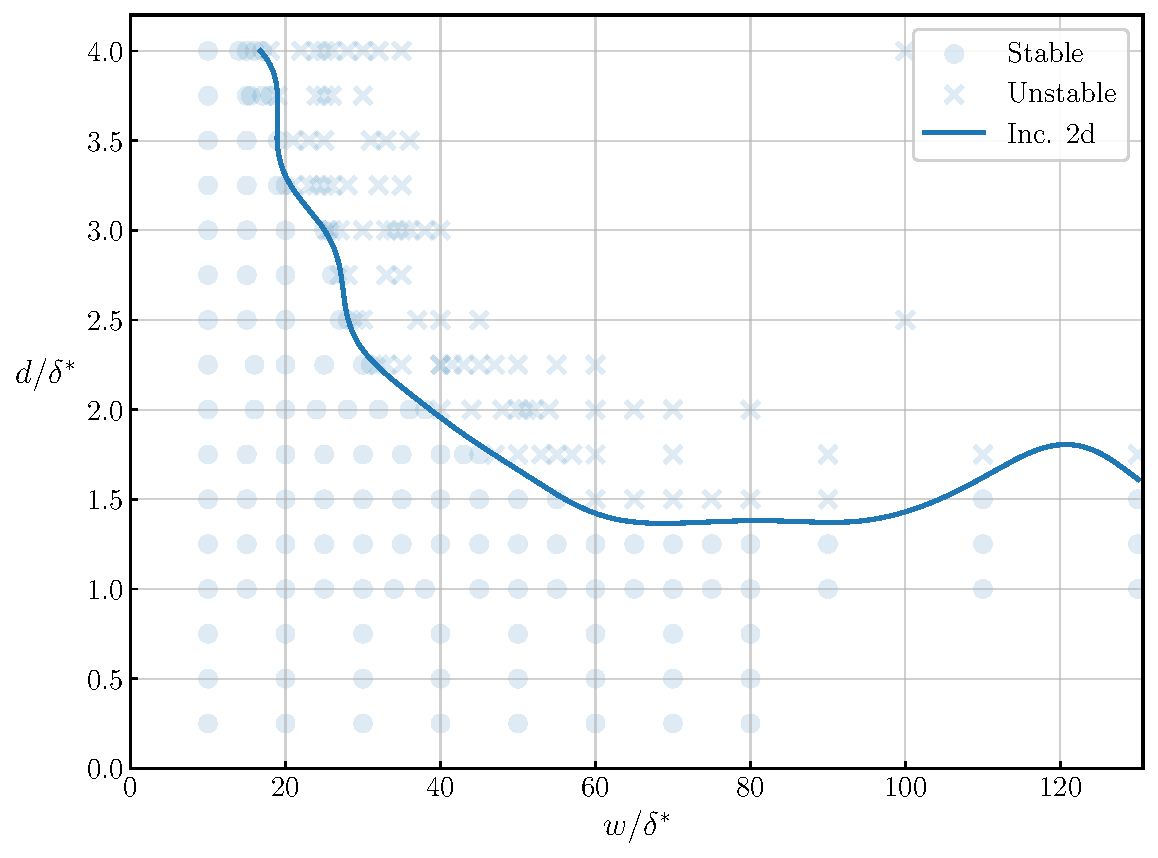
\includegraphics[width=0.75\linewidth]{../../../images/stabilityCurve.pdf}
\end{frame}

\begin{frame}
  \frametitle{3d  TS transition (d=1.5 w=80)}
  \begin{itemize}
    \item At shallow gaps the frequency of the modes at the dowstream edge of the gap getsvery close to the TS frequency regime. So it make sense.
    \item Turbulence not well resolved but the trend is clear.
    \item Mode in the cavity is 2d (the TS waves do not come from upstream).
  \end{itemize}
  \vspace{-0.25cm}
  $v$ iso-surfaces
  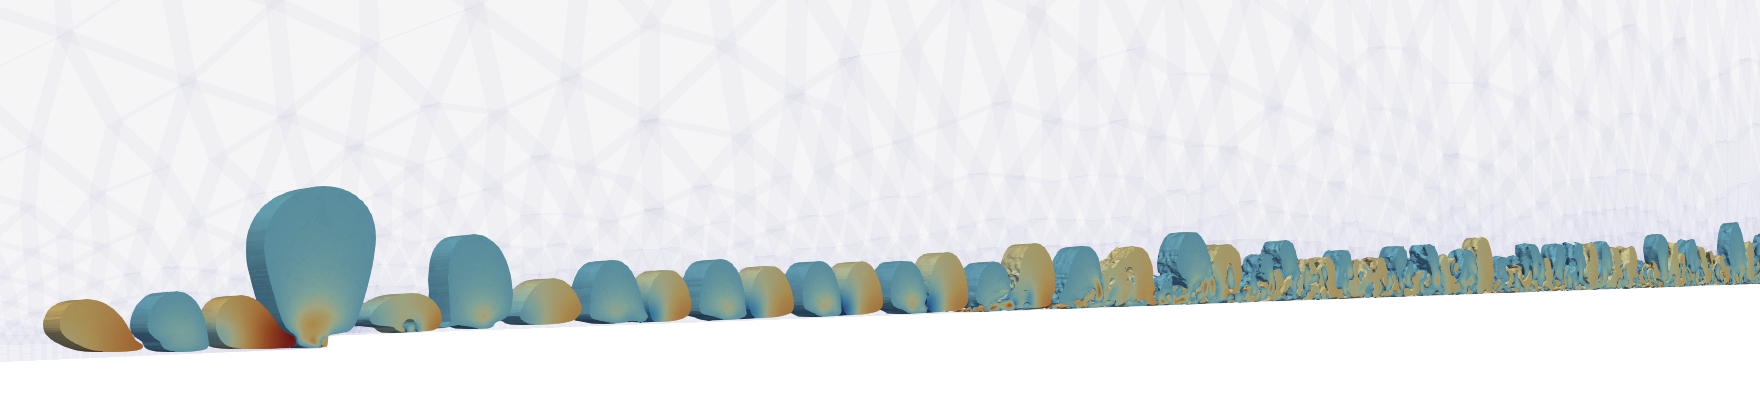
\includegraphics[width=\linewidth]{Images/d1.5_w80_tstransition_v.png} 
  $w$ contours
  
\includegraphics[width=\linewidth]{Images/d1.5_w80_tstransition_w.png} 
\end{frame}
\begin{frame}
  \frametitle{Burst of TS wave packets at shallow depths}
\begin{columns}[T] % [T] ensures correct vertical alignment
		\begin{column}{0.49\linewidth} % Left column
			\begin{itemize}
			  \item From time to time, a packet of TS waves is generated in the middle of the gap and travels downstream.
			  \item Then for some time the flow stabilizes until a new packet is generated.
			  \item This is for $d=1.5$, $w=50$ at $Ma=0.6$.
			  \item I have a video at $videos/d1.5\_w50\_comGapRe1000Ma0.6.gif$.
			\end{itemize}
		\end{column}
		\begin{column}{0.49\linewidth} % Left column
		      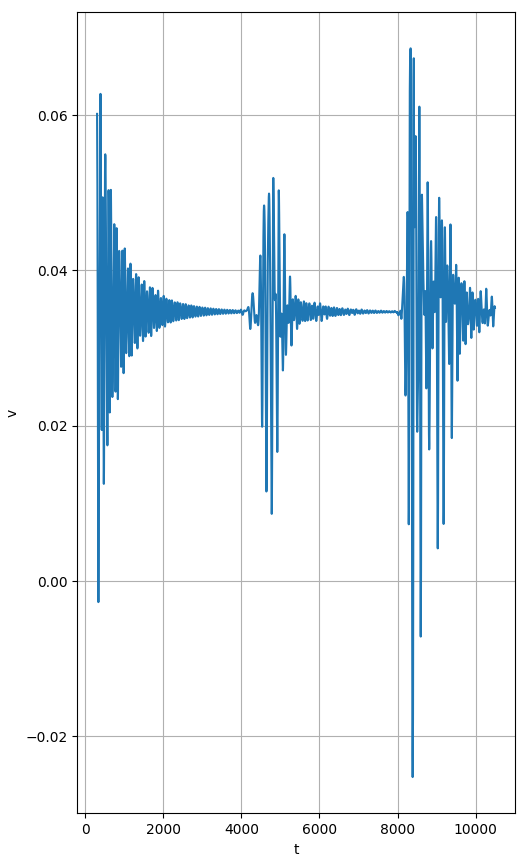
\includegraphics[width=0.6\linewidth]{Images/d1.5_w50Ma0.6_burst.png}
		\end{column}
	\end{columns}
\end{frame}
\end{document}
